\chapter{MDPs}

\subsection{MDP examples}\label{MDP-examples}
Examples of MDPs in the wild.

\hypertarget{bus-engine-replacement}{%
\paragraph{Bus engine replacement}\label{bus-engine-replacement}}

\begin{itemize}
\tightlist
\item
  \textbf{States:} Accumulated mileage of each bus (since their last
  replacement).
\item
  \textbf{Actions:} Replace bus \(i\), Y / N. If Y, what year model to
  replace with?
\item
  \textbf{Transition fn:} How the mileage of each bus changes between
  fitness checks.
\item
  \textbf{Reward fn:} Age dependent recurring cost - for repairs - and
  replacement cost.
\end{itemize}

Note: The transition function could be diagonal, or not. If diagonal
then buses are not able to effect the milage of other busses, possibly
by taking another's shift. In this case, the problem is reduced to a
contextual bandit problem (?).

\cite{Putterman2015}

\hypertarget{the-aloha-protocol}{%
\paragraph{The ALOHA protocol}\label{the-aloha-protocol}}

\begin{itemize}
\tightlist
\item
  \textbf{States:} For each terminal, is last attempt a collision.
\item
  \textbf{Actions:} The probability of each terminal attempting to send
  a new packet (if there has been a collision).
\item
  \textbf{Transition fn:} Combines terminal packets into either a
  successful transmission, or a collision.
\item
  \textbf{Reward fn:} If a packet is sent, great. If not, bad.
\end{itemize}

\cite{Putterman2015} pg 8

\hypertarget{mate-desertion-in-coopers-hawks}{%
\paragraph{Mate desertion in Cooper's
Hawks}\label{mate-desertion-in-coopers-hawks}}

\begin{itemize}
\tightlist
\item
  \textbf{States:} The product of the brood's health and mother's health
  (\([2:7] \times [2:7]\)).
\item
  \textbf{Actions:} Stay, hunt, desert.
\item
  \textbf{Transition fn:} The four developmental stages, early nestling,
  late netling, early feldgling, late feldgling. From one developmental
  stage to the next, the energy levels of the mother and brood are
  determined by the initial energy reserves, the actions taken and the
  availability of food. (this was estimated from data data gatherd by
  \ldots{})
\item
  \textbf{Reward fn:}
\end{itemize}

\cite{Putterman2015} pg 10

\hypertarget{but-whos-counting}{%
\paragraph{But who's counting?}\label{but-whos-counting}}

\begin{itemize}
\tightlist
\item
  \textbf{States:} A random number, and the value of each of five
  possible locations. Possibly none value.
\item
  \textbf{Actions:} Choose which location to add the latest random
  number.
\item
  \textbf{Transition fn:} Deterministically updates the storage location
  given the action and observed random number.
\item
  \textbf{Reward fn:} The total magnitude of the stored number, only
  given after the storage is full..
\end{itemize}

\cite{Putterman2015} pg 13

\hypertarget{diagnosing-catnip-immunity}{%
\paragraph{Diagnosing catnip
immunity}\label{diagnosing-catnip-immunity}}

\begin{itemize}
\tightlist
\item
  \textbf{States:} The truth values for immuity to an of the 4 drugs (
  Catnip / Valerian / Silvervine / Honeysuckle )
\item
  \textbf{Actions:} Choose which drug to test.
\item
  \textbf{Transition fn:} Updates the truth values with some probability
  of returning a true postive or false negative.
\item
  \textbf{Reward fn:} Minimize the cost to find a working drug.
  Catnip=\$8.96, Valerian=\$7.00, Silverine=\$17.77, Honeysuckle=\$7.99.
\end{itemize}

\begin{quote}
Bol et al 2017, as noted, provides responses for 4 drugs
(catnip/Valerian/silvervine/honeysuckle) in a large sample of cats;
responses turn out to be heavily intercorrelated, permitting the ability
to better predict responses to the catnip alternatives based on a known
response to one of the others. This becomes useful if we treat it as a
drug selection problem where we would like to find at least one working
drug for a cat while saving money, and adapting our next test based on
failed previous tests.
\end{quote}

\begin{quote}
If they were not intercorrelated, one would simply minimize expected
loss in a greedy fashion, starting with catnip etc; but as they are
intercorrelated, now a drug has both direct value (if the cat responds)
and value of information (its failure gives evidence about what other
drugs that cat might respond to), which means the greedy policy may no
longer be the optimal policy.
\end{quote}

\href{https://www.gwern.net/Catnip\#optimal-catnip-alternative-selection-solving-the-mdp}{gwern
on Catnip}

This one is interesting. The four actions effect only the four state
element-wise. But our knowledge that certain immunities are correlated
make it possible to intelligently guess which tests should be performed.

\hypertarget{ad-targeting}{%
\paragraph{Ad targeting}\label{ad-targeting}}

\hypertarget{youtube-recommendation}{%
\paragraph{Youtube recommendation}\label{youtube-recommendation}}

\hypertarget{salamon-harvesting}{%
\paragraph{Salamon harvesting}\label{salamon-harvesting}}

\begin{itemize}
\tightlist
\item
  \textbf{States:} The size of the salamon population.
\item
  \textbf{Actions:} The size of the salamon population to be left to
  spawn.
\item
  \textbf{Transition fn:} Given the number left to spawn, it returns the
  size of the salamon population in the next season.
\item
  \textbf{Reward fn:} The size of salamon population harvested.
\end{itemize}

YOu might call this MDP a one dimensional MDP, as there is only a single
dimension that is acted up, is transitioned, is rewarded\ldots{} More
salamon

\href{http://www.it.uu.se/edu/course/homepage/aism/st11/MDPApplications1.pdf}{Real
applications of MDPs}

\hypertarget{fire-engine-allocation}{%
\paragraph{Fire engine allocation}\label{fire-engine-allocation}}

\begin{itemize}
\tightlist
\item
  \textbf{States:} The magnitude of a fire. The type of alarm. And the
  total number of first and second fire engines already deployed.
\item
  \textbf{Actions:} Whether to send more fire engines.
\item
  \textbf{Transition fn:} Given the number of fire engines fighting the
  fire, and the fires type / magnitude, the building may be destroyed or
  saved. Fire may start at anytime, in a random location throughout the
  city.
\item
  \textbf{Reward fn:} Damage incurred by the fires.
\end{itemize}

\href{http://www.it.uu.se/edu/course/homepage/aism/st11/MDPApplications1.pdf}{Real
applications of MDPs}

Other possible MDPs?

\begin{itemize}
\tightlist
\item
  An animal stockpiling food?!
\item
  Robotics / movement
\end{itemize}

\begin{center}\rule{0.5\linewidth}{\linethickness}\end{center}

More Refs

\begin{itemize}
\tightlist
\item
  http://www.it.uu.se/edu/course/homepage/aism/st11/MDPApplications1.pdf
\item
  https://www.worldscientific.com/worldscibooks/10.1142/p809
\end{itemize}


\subsection{Other properties of the polytope}



\subsubsection{Distribution of policies}

A potentially interesting question to ask about the polytopes is how the
policies are distributed over the polytope. To calculate this
analytically, we can use the probability chain rule:
\(p(f(x)) = \mid \det\frac{\partial f(x)}{\partial x}\mid^{-1}p(x)\).
Where we set \(f\) to be our value functional and \(p(x)\) to be a
uniform distribution.

\begin{figure}
\centering
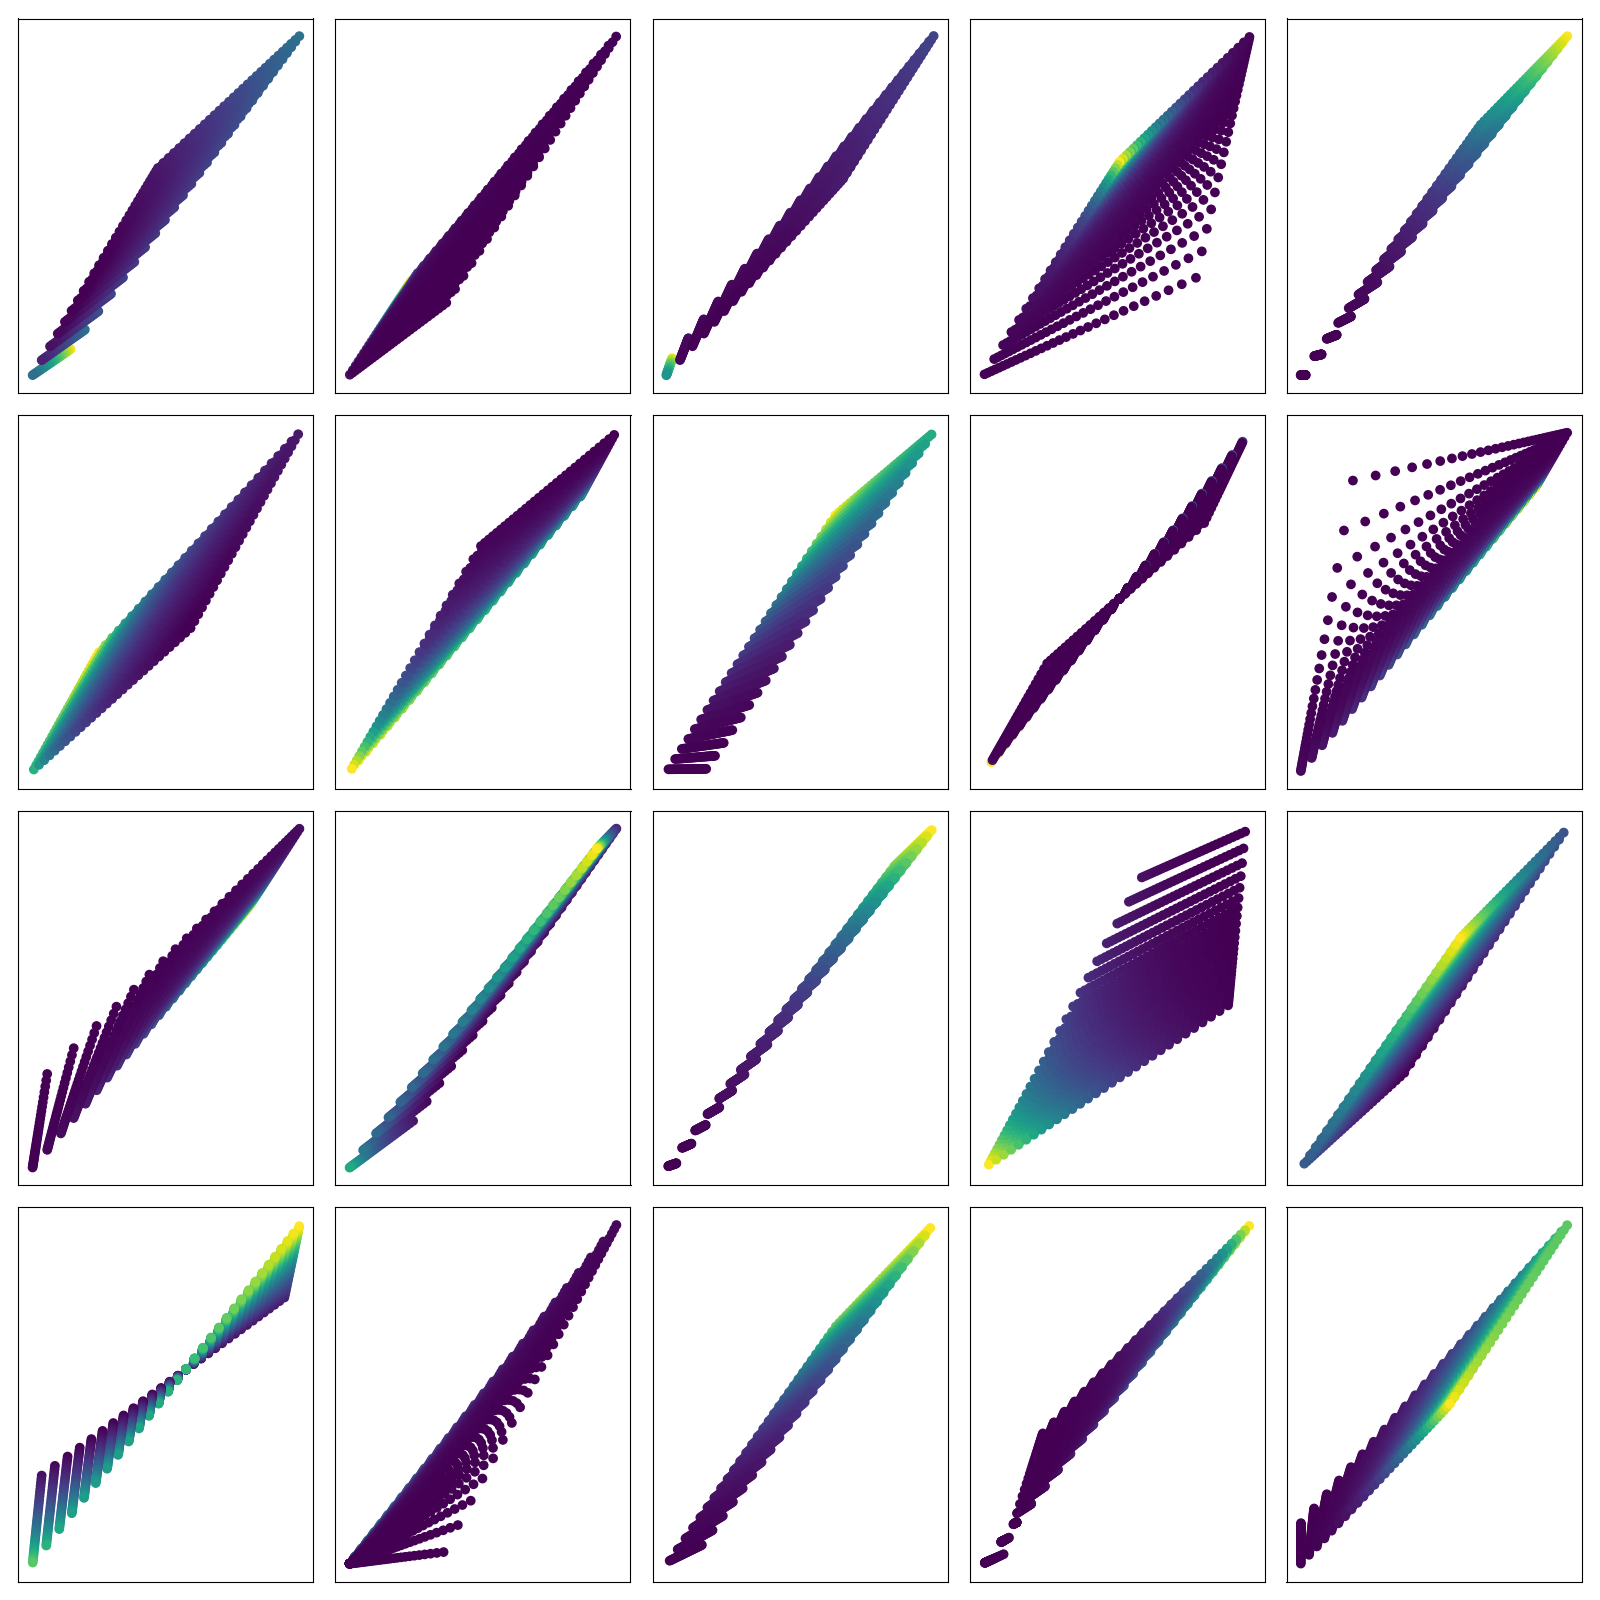
\includegraphics[width=0.5\textwidth,height=0.5\textheight]{../../pictures/figures/polytope_densities.png}
\caption{`2-state 2-action MDPs. We have visualised the likelihood of
values under a uniform on policies. They are coloured by density.
Lighter colour is higher probability'}
\end{figure}

\begin{itemize}
\item
  \textbf{Observation} In some polytopes, many of the policies are close
  to the optimal policy. In other polytopes, many of the policiesare far
  away from the optimal policy. \textbf{Question} Does this make the MDP
  harder or easier to solve? \textbf{Intuition} If there is a high
  density near the optimal policy then we could simply sample policies
  and evaluate them. This would allow us to find a near optimal policy
  with relative easy.
\item
  \textbf{Observation} The density is always concentrated / centered on
  an edge.
\item
  \textbf{Question} how does the entropy of the distribution change
  under different gamma/transitions/rewards\ldots{}?
\end{itemize}

\paragraph{An MDPs Entropy}

(\emph{the goal is to understand what makes some MDPs harder to solve
than others})

We can visualise polytopes in 2D, but we struggle in higher dimensions.
However, it is possible to use lower dimensions to gain intuition about
metrics and carry that intuition into higher dimensions. A potential
metric of interest here is the entropy of our distribution, (and / or
the expected distance from the optima) to give intuition about
unimaginable MDPs.

\begin{align}
M &\to \{P, r, \gamma\} \tag{a MDP}\\
H(M) &:= \mathop{\mathbb E}_{\pi\sim\Pi}\Big[-\log p(V(\pi)) \Big]\\
&= \mathop{\mathbb E}_{\pi\sim\Pi}\Big[-\log(\mid \det\frac{\partial V(\pi)}{\partial \pi}\mid^{-1}p(\pi)) \Big] \\
&= \mathop{\mathbb E}_{\pi\sim\Pi}\Big[-\log(\mid \det \frac{r}{(I-\gamma P \pi)^2}\mid^{-1}p(\pi)) \Big] \\
\end{align}

What does this tell us? \textbf{???} A MDP with a low entropy tells us
that many of the policies are in a corner of the polytope. But the
`hardness' of the MDP depends on which corner these policies are
concentrated in. Rather we could use the value of each policy to give
information about the location of the policy.

\begin{align*}
\mu(M) &:= \mathop{\mathbb E}_{\pi\sim\Pi}\Big[V(\pi) \Big]\\
\end{align*}

What does this tell us? The expected value of a policy. Thus, a quantity
of interest might be the expected suboptimality of a policy,
\(s = V(\pi^{* })-\mu(M)\). This tells us how far away the optimal
policy is from the center of mass of the polytope.

\textbf{Conjecture:} If an MDP has suboptimality
\(s \le \frac{\sigma_{MDP}}{D}\) then it is possible to find a
\(\epsilon\) optimal policy with \(\mathcal O(n)\) samples. (but
sampling in high dimensions always scales badly?!)

\textbf{Experiment:} Correlate the properties of \(P, r\) with entropy.
Or find derivative wrt \(P, r\). What properties of \(P, r\) yield
easily solvable MDPs?

NOTE:

\begin{itemize}
\item
  What about the variance of the MDP? What does that tell us?
\item
  How does a uniform distribution on a simplex behave in high
  dimensions? Does it become more likely to sample from the center? Less
  likely to sample from vertices??
\item
  In most cases, this is unlikely to work. A high dimensional polytope
  \ldots{} low density everywhere!?
\end{itemize}


\subsubsection{Discounting}

How does the shape of the polytope depend on the discount rate? Given an
MDP, we can vary the discount rate from \(0\) to \(1\) and explore how
the shape of the value polytope changes.

\begin{figure}
\centering
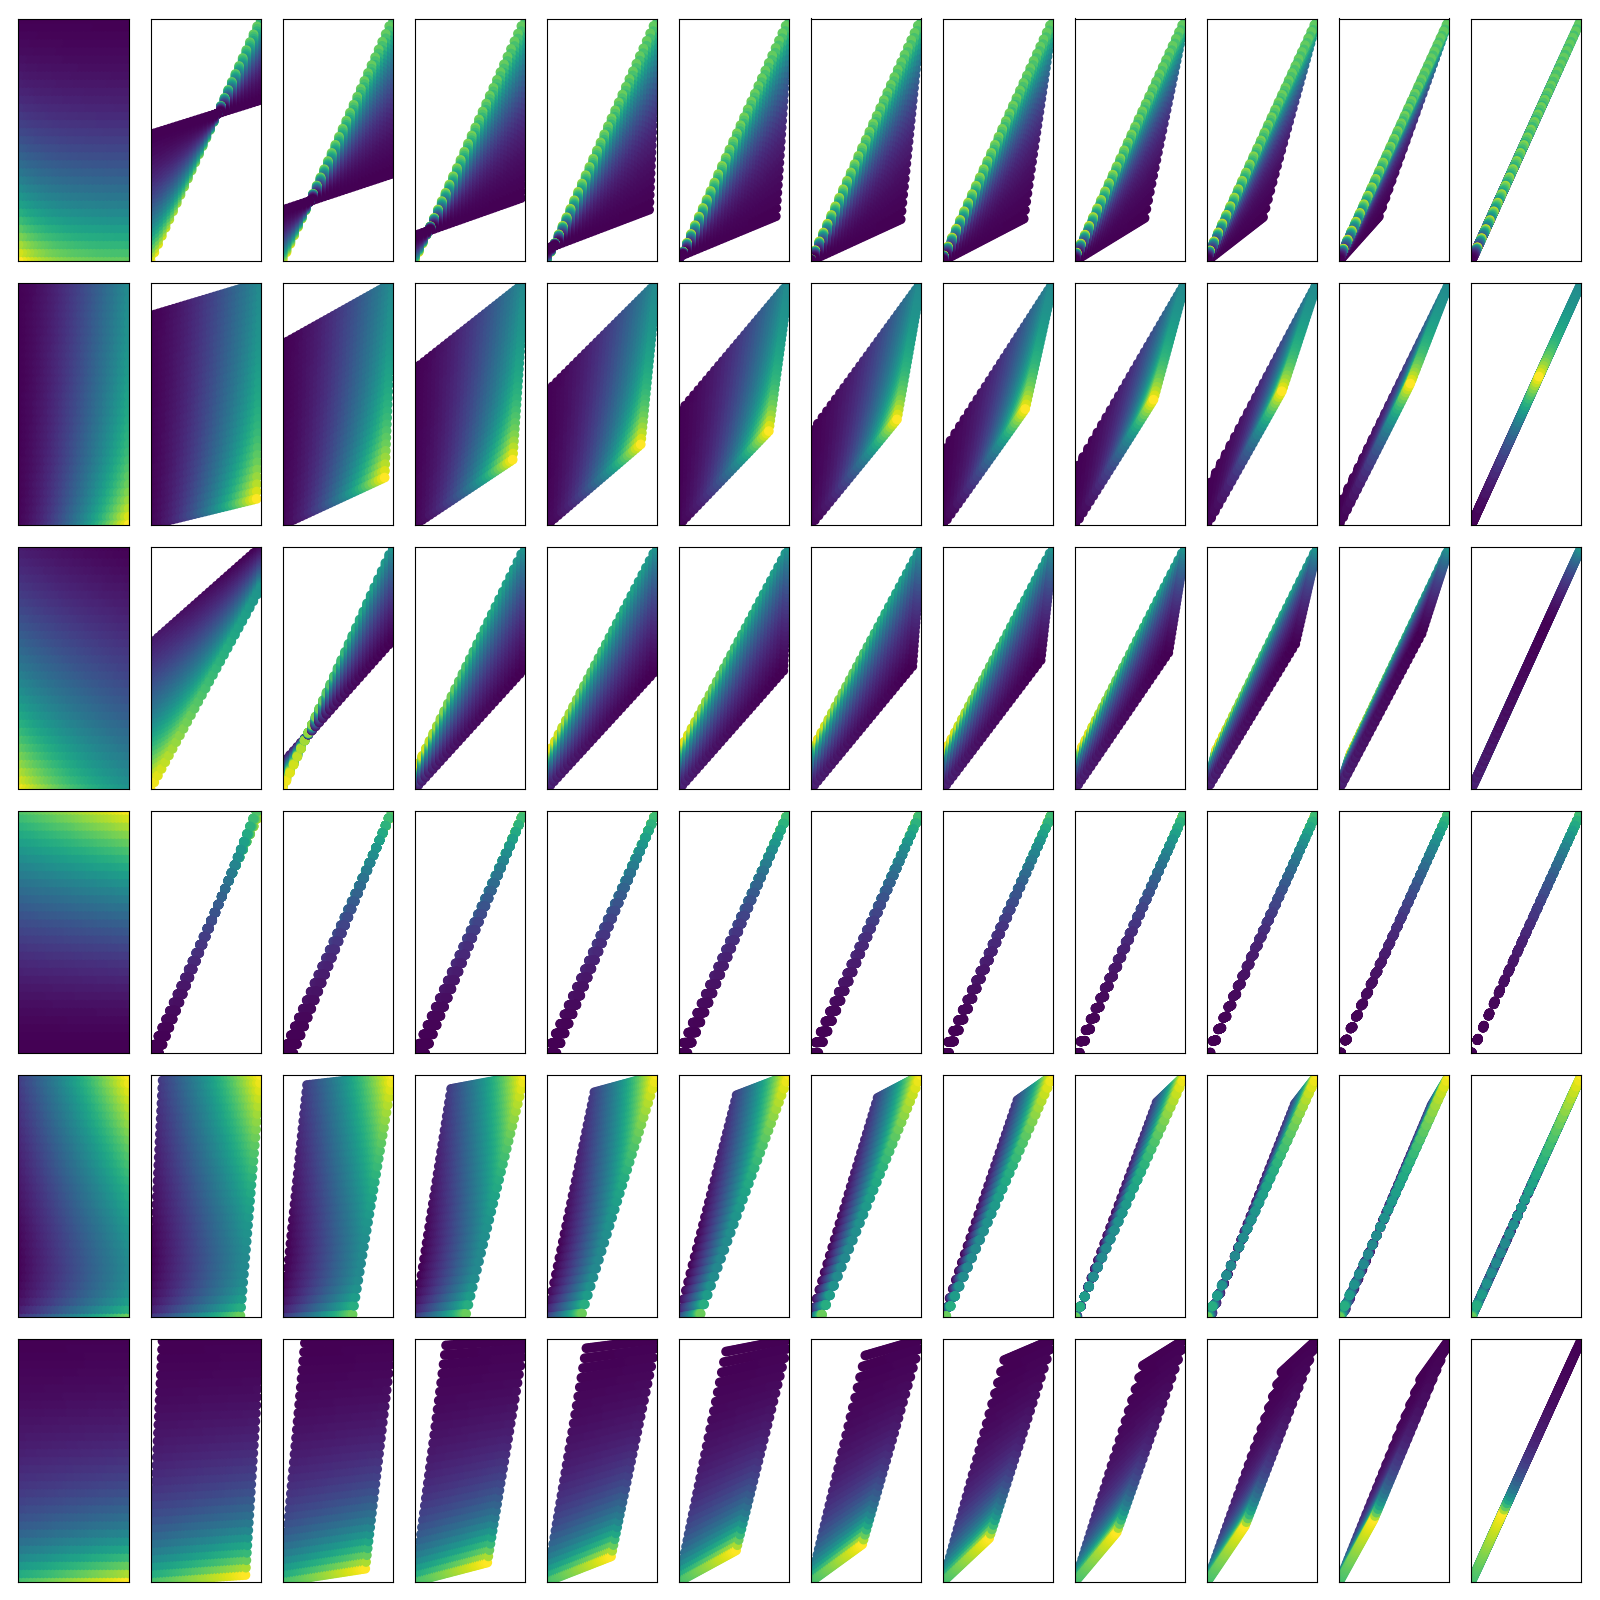
\includegraphics[width=0.5\textwidth,height=0.5\textheight]{../../pictures/figures/discounts.png}
\caption{`Here we have shown a few different 2 state, 2 action, MDPs and how their polytopes change with changes in discount rate.'}
\end{figure}

\begin{itemize}
\item
  \textbf{Observation} As \(\gamma \to 1\), all the policies are
  projected into a 1D space? \textbf{Question} Does this make things
  easier to learn? \textbf{Intuition} Orderd 1D spaces are easy to
  search.
\item
  \textbf{Observation} The tranformation that changing the discount
  applies is quite restricted. They are not generally non-linear, but
  appear `close to linear', but not quite. \textbf{Question} What is the
  set of functions /transformations that the discount can apply?
\end{itemize}

\subsection{Derivation of derivative}

\begin{align}
V(\pi) &= (I − \gamma P_{\pi})^{−1}r_{\pi} \\
&= (I − \gamma P\cdot \pi)^{−1}r\cdot \pi \\
\frac{\partial V}{\partial \pi} &= \frac{\partial}{\partial \pi}((I-\gamma P_{\pi})^{-1} r_{\pi}) \\
&= (I-\gamma \pi P)^{-1} \frac{\partial \pi r}{\partial \pi}+   \frac{\partial (I-\gamma \pi P)^{-1}}{\partial \pi}\pi r\tag{product rule} \\
&= (I-\gamma \pi P)^{-1} r + -(I-\gamma \pi P)^{-2} \cdot -\gamma P\cdot \pi r\\
&= \frac{r}{I-\gamma \pi P} + \frac{ \gamma P\cdot \pi r}{(I-\gamma \pi P)^2}\\
&= \frac{r(I-\gamma \pi P) + \gamma P \pi r}{(I-\gamma \pi P)^2} \\
& = \frac{r}{(I-\gamma P \pi)^2} \\
\end{align}

TODO. Annotate. Add numbers and explain.



\section{What are the properties of the polytope?}

\begin{displayquote}
  \textit{How is the structure of the RL problem reflected in geometry?}
\end{displayquote}

How is the shape of the polytope determined by the Bellman equation?
If we look at the polytope, we see that;
\begin{itemize}
\tightlist
\item
  All the edges have positive gradients
\item
  All the edges are linear
\item
  Non-convex
\end{itemize}


% An increase in the value of state one, can, at worst, do nothing for state two, aka a
% flat line, either horizontal or vertical. But if the value of the other state
% increases and there is a non zero chance of transitioning to that state, from your current state,
% then that will increase the value of your current state.
% This explains why the edges of the polytope by be aligned with the positive orthant, they slant upward.

\begin{align}
\hat V(s_1) = V(s_1)P(s_1|s_1, a)\pi(a|s_1) + V(s_2)P(s_2|s_1, a)\pi(a|s_1)
\end{align}

\begin{itemize}
\tightlist
\item
If $V(s_1)$ increases then $\hat V(s_1)$ must increase...
\item
If $V(s_2)$ increases then $\hat V(s_1)$  either increases or stays the same. As $P(s_2|s_1, a)\pi(a|s_1) \ge 0$
\end{itemize}

\section{Policies in high dimensions}



\begin{figure}
\centering
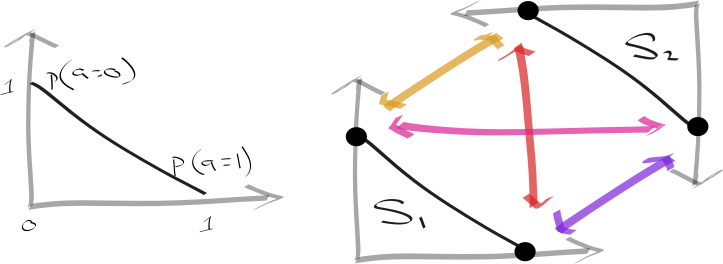
\includegraphics[width=1\textwidth,height=0.25\textheight]{../../pictures/drawings/2-state-2-action-simplices.png}
\caption{Imagine what the geometry of the space of policies in the two state, two action MDP. A policy tells us what actions should be taken when in a given state. Therefore, there will be \(|A| \times |S|\) entries in the policy. However, because the policy returns a distribution over actions, the true dimensionality of the policy is \((|A| -1) \times |S|\). Which in the two state, two action case equals 2D.}
\end{figure}

\begin{figure}
\centering
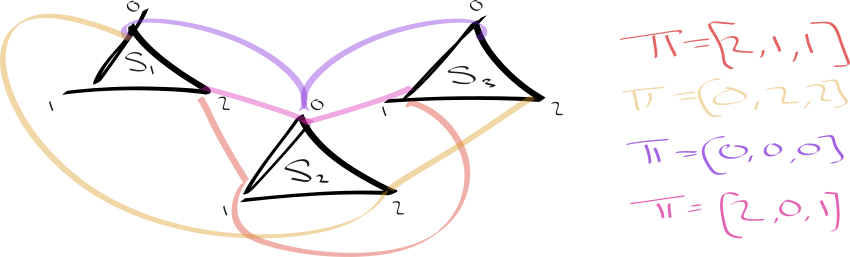
\includegraphics[width=1\textwidth,height=0.25\textheight]{../../pictures/drawings/3-state-3-action-simplices.png}
\caption{Let's \textit{try} to gain some intuition about the space of policies in higher dimensions.
For each state, we have a distribution (on a simplex), over the possible actions.}
\end{figure}


\section{Model search}

Lastly, we can search through possible models, $P, r$. Models that fit the
observations we make. That is policy $\pi_i$ has a value $V^{\pi_i}$.

\begin{displayquote}
  \textit{This model predicts that the ??? policy is of high value.
  However, when I tried this policy, I ended up with ...?
  My model must be wrong.}
\end{displayquote}

Here the parameters are composed to two independent parts, the transition function
and the reward function.

\begin{align}
\tilde P^{* }, \tilde r^{* } = \mathop{\text{argmin}}_{\tilde P, \tilde r} \int_{\Pi} \parallel V^{\pi}_{P, r} -V^{\pi}_{\tilde P, \tilde r} \parallel_\infty
\end{align}

While it is nice to have $\tilde P^{* }, \tilde r^{* }$, the ultimate goal of
solving a MDP is to find the optimal policy. ...!?!?

\subsubsection{Relationship to model based RL}

Most model-based learning approaches to RL ... next step prediction (refs!!!)
This algorithm only focuses on relevant features of the state space.

Consider a problem where the reward is only determined by the first feature of the state. We can add $n$ extra, useless, features.
The model based learner will spend resources on attempting to build a good predictor of those $n$ features.

Sample efficient. You only need to collect data for the $m$ policies we are matching under.
Once that has been done, the optimisation problem is easily solved!?

Model iteration. Model invariant transforms. Pick a policy. Falsify it,
and this falsify all models that yield the same optimal policy.

\begin{figure}
\centering
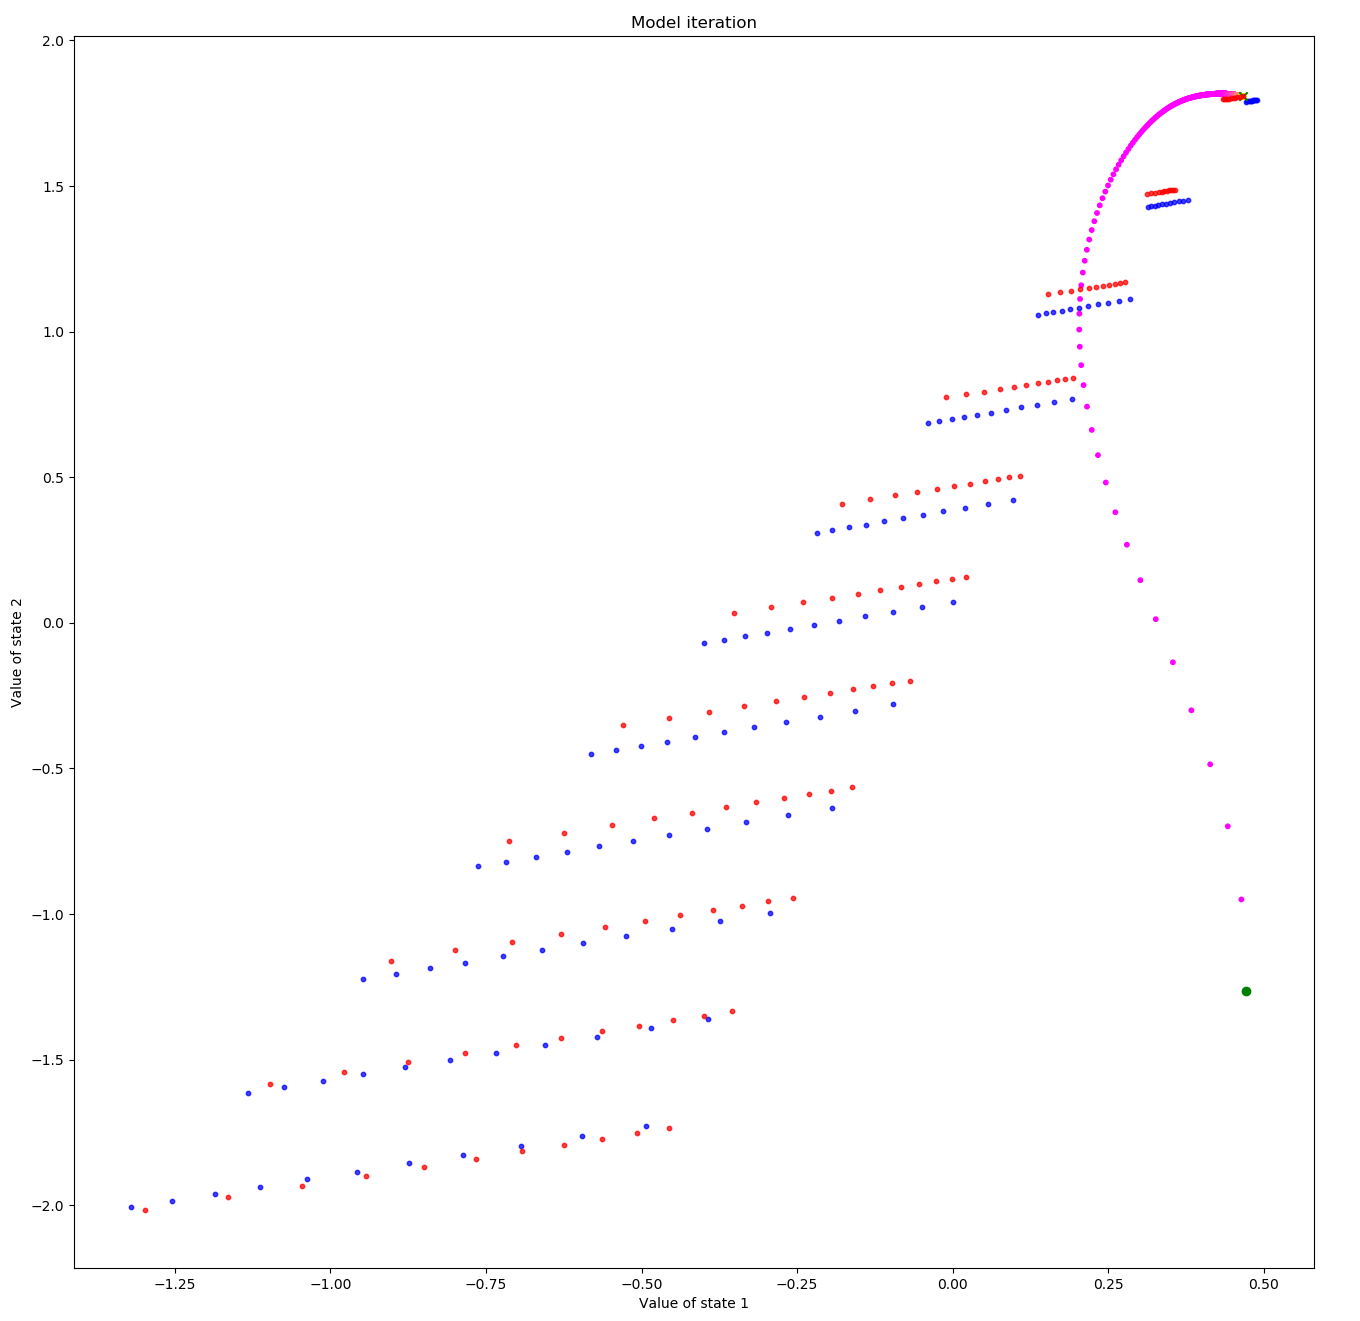
\includegraphics[width=0.5\textwidth,height=0.5\textheight]{../../pictures/figures/model_iteration.png}
\caption{Blue shows the value of policies when evaluated under the true model, $P, r$,
and Red shows the estimated value of policies when evaluated under the learned model at convergence, $\tilde P, \tilde r$.}
\end{figure}


Related to AWR? https://arxiv.org/pdf/1910.00177.pdf
